\section{Future Work}\label{future-work}

Ideally, our work would have resulted in a complete taxonomy of software
testing terminology based on the literature. Unfortunately, we were not able to
fully accomplish this due to time constraints. With more time, we would
continue iterating over undefined terms (\Cref{future-undef-terms}) and
investigate terms we \emph{expected} to find but never did
(\Cref{future-miss-terms}). We could also look for other approach data that
never arose from our methodology (\Cref{future-app-data}).
Additionally, there is much more work we could do to analyze our data on the
software testing literature, such as improving our visualizations
(\Cref{future-rel-vis}) and detecting (and identifying!)\ more classes of flaws
(\Cref{future-detect-flaws}).

\subsection{Iterating Over Undefined Approaches}\label{future-undef-terms}

As we explain in \Cref{undef-terms}, our methodology includes performing
miniature literature reviews on undefined test approaches to record their
missing definitions (and any relations). We were able to do this for the
following approaches, although some are out of scope, such as \acf{emsec}
testing, aspects of \acf{orthat} and loop testing (see \Cref{hard-test}),
and HTML testing (see \Cref{lang-test}). We investigate the following terms
(and their respective related terms) in the sources given:
\input{build/undefTerms}

Applying our procedure shown in \Cref{fig:recAppFlowchart} to these sources
uncovers \the\numexpr \TotalAfter - \TotalBefore\relax\ new approaches and
\the\numexpr \TotalAfter - \UndefAfter - \TotalBefore + \UndefBefore\relax\ new
definitions. These definitions are either for existing undefined approaches or
new uncovered approaches; while not every new approach is presented alongside
a definition, if we assume that each of these definitions is for a new approach,
we can deduce that about \the\numexpr 100 - 100 * (\UndefAfter - \UndefBefore) /
(\TotalAfter - \TotalBefore)\relax\% of added test approaches are defined. This
indicates that this procedure leads to a higher proportion of defined terms
(\the\numexpr 100 - 100 * \UndefBefore / \TotalBefore\relax\% vs.~%
\the\numexpr 100 - \undefPerc\relax\%), as shown in
\Cref{fig:undefPies}, which helps verify that our procedure constructively
uncovers \emph{and} defines new terminology. With repeated iterations, this
ratio would approach 100\%, resulting in a (plausibly) complete taxonomy. We
give the full list of undefined test approaches in \Cref{app-undef-terms} for
completeness.

\begin{figure*}[hbtp!]
    \begin{subfigure}[c]{0.35\linewidth}
        \centering
        \begin{tikzpicture}[thick, scale=0.7, every label/.style={align=left, scale=0.7}]
            \pie[text=inside, sum=auto, color={blue!60, orange!60}]{
                {\the\numexpr \TotalBefore - \UndefBefore\relax}/,
                {\the\UndefBefore}/
            }
        \end{tikzpicture}
        \caption{The \the\TotalBefore{} approaches before investigating undefined terms.}
        \label{fig:undefPiesBefore}
    \end{subfigure}
    \hfill
    \begin{subfigure}[c]{0.35\linewidth}
        \centering
        \begin{tikzpicture}[thick, scale=0.7, every label/.style={align=left, scale=0.7}]
            \pie[text=inside, sum=auto, color={blue!60, orange!60}]{
                {\the\numexpr \TotalAfter - \UndefAfter\relax}/,
                {\the\UndefAfter}/
            }
        \end{tikzpicture}
        \caption{The \the\TotalAfter{} approaches after investigating undefined terms.}
        \label{fig:undefPiesAfter}
    \end{subfigure}
    \hfill
    \begin{subfigure}[c]{0.2\linewidth}
        \centering
        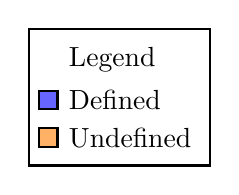
\begin{tikzpicture}
            \matrix [thick, draw=black] {
            \node[label=right:{Legend}] {}; \\
            \node[thick, shape=rectangle, draw=black, fill=blue!60,   label=right:{Defined}](0) {}; \\
            \node[thick, shape=rectangle, draw=black, fill=orange!60, label=right:{Undefined}](1) {}; \\
            };
        \end{tikzpicture}
    \end{subfigure}
    \caption{Breakdown of how many test approaches are undefined.}
    \label{fig:undefPies}
\end{figure*}

\clearpage
\subsection{Investigating Missing Test Approaches}\label{future-miss-terms}
In addition to these undefined approaches, some do not appear in
the literature at all! While most arise as a result of our
snowballing approach, we each have preexisting knowledge of what test
approaches exist (a form of experience-based testing, if you will).
Test approaches that arise independently of snowballing may
serve as starting points for continued research if we do not find them in
the literature using our iterative approach. The following terms come from
previous knowledge, conversations with colleagues, research for other
projects, or ad hoc cursory research to see what other test approaches exist:
\newline

\begin{minipage}{0.92\textwidth}
    \centering
    \begin{multicols}{2}
        \begin{enumerate}
            \item Chaos engineering
            \item Chosen-ciphertext attacks
            \item Concolic testing
            \item Concurrent testing\footnote{This seems to be distinct from
                      ``concurrency testing''.}
            \item Context-driven testing
            \item Destructive testing
            \item Dogfooding
            \item Implementation-based testing\footnote{This may or may not be
                      distinct from ``implementation-oriented testing.''}
            \item Interaction-based testing
            \item Lunchtime attacks\footnote{In previous meetings, Dr.~Smith
                      mentioned that with the number of test approaches that
                      suggest that people just like to label everything as
                      ``testing'', he would not be surprised if something
                      like ``Monday morning testing'' existed. While
                      independently researching chosen-ciphertext attacks
                      out of curiosity, this prediction of a time-based
                      test approach came true with ``lunchtime attacks''.}
            \item Parallel testing
            \item Property-based testing
            \item Pseudo-random bit testing
            \item Rubber duck testing
            \item Sanity testing
            \item Scream testing
            \item Shadow testing
            \item Situational testing
        \end{enumerate}
    \end{multicols}
\end{minipage}

\subsection{Filling in Other Approach Data}\label{future-app-data}
Definitions are not the only piece of information that can be missing for some
test approaches. As mentioned in \Cref{syn-conds}, some test approaches are
``orphans'' without a parent-child relation \emph{or} a significant synonym
relation. To reduce clutter, we omit these from our visualizations, but
iterating over these orphan approaches to find any relations in the literature
could provide a more complete picture of the state of software testing.%
\qtodo{Should I add this to our methodology if we didn't apply it?} We give the
full list of these orphans in \Cref{app-orphan-terms} for completeness.

Additionally, some test approaches are not given one of the categories we use
in \Cref{tab:ieeeCats}. Following our methodology, we assign each category the
``default'' category ``Approach'' until we uncover a more specific one as
shown in \Cref{fig:recAppFlowchart}. Assuming these categories are complete
(which they may not be; see \Cref{alt-criteria}), we could either decide on an
appropriate category for each uncategorized approach or further investigate
these terms to see if they are categorized by other sources. We give the
full list of test approaches with the general category of ``Approach'' in
\Cref{app-uncat-terms} for completeness.

\subsection{Improving Relation Visualizations}\label{future-rel-vis}
As described in \Cref{app-rel-vis}, we currently visualize the relations
between test approaches by identifying relations that are notable to include.
We then add a line for each relation to each relevant \LaTeX{}
\texttt{digraph} to render them. While sufficient for the purposes of this
research, this was mainly done as a proof of concept\thesisissueref{67} and
could be done more robustly and efficiently. The use of a more elaborate tool
could make these visualizations interactive, making these dense overviews more
usable and accessible.\qtodo{Should I cite Dr.~Paige here at all?}

\subsection{Detecting More Flaws}\label{future-detect-flaws}
In addition to the classes of flaws we \emph{do} detect automatically, we could
detect many more if time permitted. We currently detect parent-child relations
that violate irreflexivity (see \Cref{autoSelfPar}) which can be thought of as
cycles with length $n=1$. Since parent-child relations should also be
transitive (see \Cref{par-chd-rels}), cycles of \emph{any} size are flaws.
Given the current way we generate visualizations of these relations (see
\Cref{app-rel-vis}), detecting cycles where $n=2$ would be straightforward: if
a parent-child relation \emph{and} its inverse (i.e., \texttt{A~->~B} and
\texttt{B~->~A} for test approaches with labels \texttt{A} and \texttt{B}) both
exist in the generated \LaTeX{} file for a visualization, (at least) one of
these parent-child flaws is incorrect since they contradict each other and we
have found a cycle. The main reason this would be time-consuming would be
deciding on how to format these findings, writing code to do so automatically
for use in this \docType{}, and resolving any issues that arise during this
process. Detecting larger cycles would also be possible but would likely
require the use of an additional tool to analyze the graph of parent-child
relations; this would likely be done alongside improving these visualizations
in general (see \Cref{future-rel-vis}).

Unfortunately, writing code to detect flaws is only half the battle. First, we
need to identify classes of flaws we even want to detect, which may never be
complete as new test approaches emerge with potentially new relations. The
classes of flaws we detect emerged over time based on our observations of the
literature. For example, our understanding of the ``standard'' test approach
categories described in \Cref{cats-def} led to us being able to detect
approaches that are categorized inconsistently in \Cref{cats,multiCats-full}.
Performing more thorough analysis, both on the literature and on our collected
data, will likely reveal more classes of flaws that can be tracked
automatically but is infeasible for the purposes of this \docType{}.
